%Paulin VIOLETTE
%Si t'as pas bossé sur l'interface utilisateur t'y touche pas.
%Sauf si la personne dont le nom est écris en haut te dis d'y toucher.
%Deso Paulin moi j'y ai touché
\chapter{Interface Utilisateur}

\section{Présentation}

%Mettre l'image de ma super interface grave stylé
\begin{figure}[h]
  \centering
  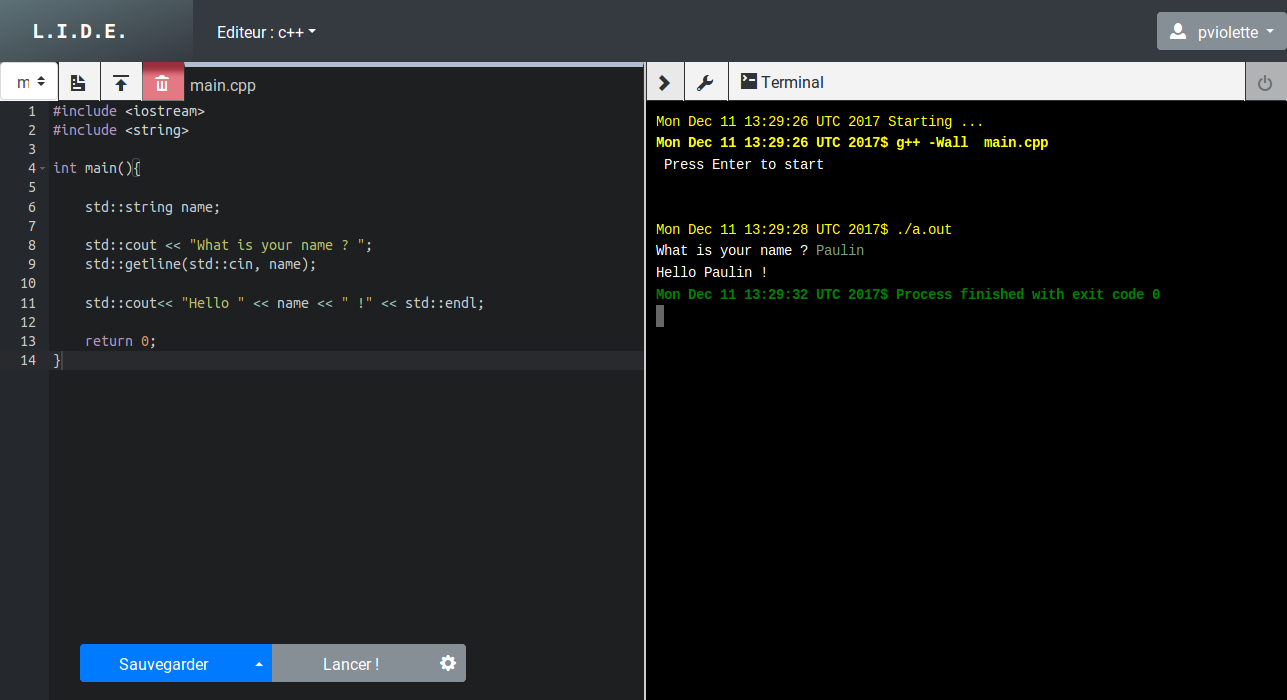
\includegraphics[width=0.8\textwidth]{./img/frontend/example1.png}
  \caption{Interface utilisateur en utilisation}
  \label{}
\end{figure}

Une fois l'utilisateur connecté, il est redirgigé vers l'interface de l'application : un éditeur de texte et une console.
L'interface est divisée en quatre parties :
\begin{itemize}
  \item La barre de navigation, contenant les liens vers les autres parties du site (gestion de compte...)
  \item La barre d'outils, qui contient des contrôles spécifiques à l'application
  \item L'editeur, implémenté par le plugin Ace
  \item La console, implémentée par le plugin jqconsole
\end{itemize}

\section{Outils utilisés}

%Blabla HTML/CSS/JS, generateur de template twig, Framework bootstrap
%Utilisation de jquery
%Editeur ace
%SweetAlert2 pour les alertes trop swag
%JQConsole vite zef parceque c'est valou qui l'a fait

\subsection{Organisation des templates TWIG}

\section{Environnement de Développement}

\subsection{Gestions des langages}
Blabla DB changement de langage

\subsection{Éditeur de texte}
Tres court parce que y'a pas grand chose à dire

\subsection{Personnalisation}

\begin{figure}
\centering
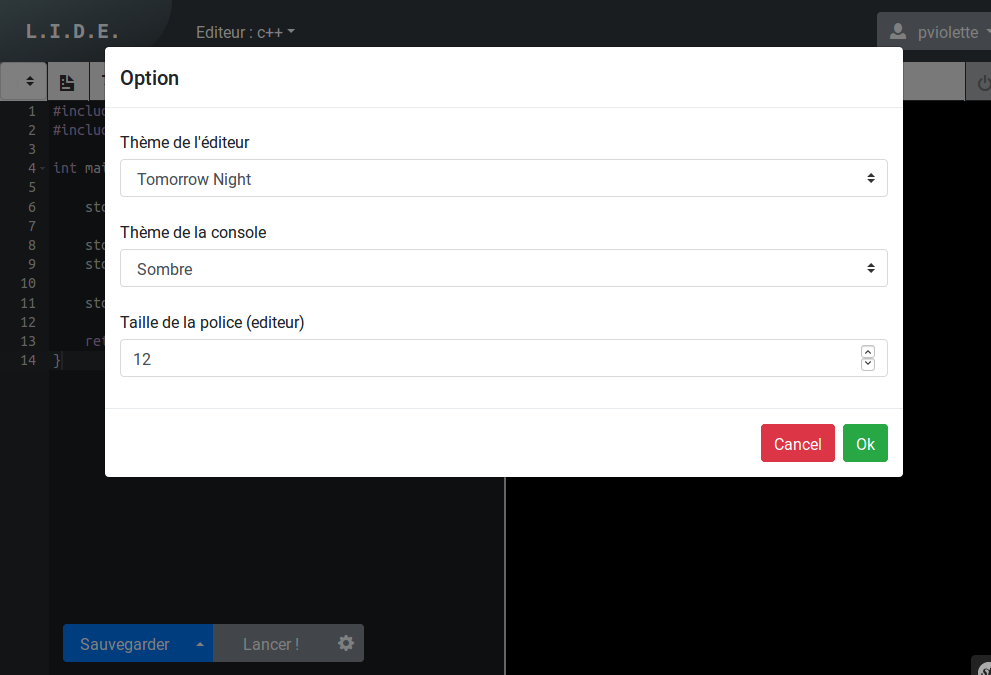
\includegraphics[width=0.8\textwidth]{./img/frontend/example_personnalisation.png}
\caption{Formulaire permettant la personnalisation de l'interface}
\end{figure}

\subsection{Gestions des fichiers}
Tel un véritable EDI, notre application permet la gestion de multiples fichiers. Cette gestion est effectué sur le navigateur, par du javascript.

\subsubsection{Stockage des fichiers et changement de fichier en cours d'édition}

Chaque fichier est représenté en JS sous la forme d'un prototype 


\section{Compilation et exécution}
Ce titre pu

\subsection{Formulaire}

SS de mon formulaire trop swag

\subsection{Terminal}

\par La mise en place de la console proposait deux options : soit la création d'une vue ad-hoc soit l'intégration d'une vue déjà existante.

\par Notre choix s'est vite tourné vers l'intégration d'une vue déjà existante. La création d'une vue nous aurait certes donné une modularité de la console en ce qui concerne les modifications mais, la console une fois implémentée n'a pas nécessairement besoin de mofications.

\par Après étude de rentabilité, nous avons décidé d'implémenter la vue JQConsole \footnote{https://github.com/replit/jq-console} qui correspondait exactement à nos besoins. En plus d'être esthétique, son code source était placé sous licence libre et toutes les fonctions qui nous étaient nécessaires étaient déjà implémentées. L'inconvénient principal est que la modification du code source peut se montrer compliqué, celui-ci étant rédigé en CoffeeScript et étant assez compliqué.

\par Nous n'avions donc plus qu'à intégrer la vue JQConsole à notre interface et faire appel aux bonnes fonctions (notamment JQConsole.Write qui permet d'afficher du texte dans la console et JQConsole.Prompt qui permet de lire du texte) pour obtenir notre console.
